\chapter{Blade Element Method}

\section{Coordinate Systems}

\subsection{Shaft-Rotating Axis System}

Origin of the Shaft-Rotating Axis System is coincident with the rotor hub center and rotates together with the rotor shaft. The z-axis it is coincident with the rotor shaft axis and points upwards, the x-axis points toward blade trailing edge and the y-axis completes a right-handed coordinate system.

Please notice that y-axis is positive toward blade tip for counter-clockwise rotors while it is negative toward blade tip for clockwise rotors.

\subsection{Blade-Span Axis System}

Origin of the Blade Axis System is coincident with the point of intersection of flapping and feathering hinge axes. The x-axis lies on XY plane of the Rotor Axis System and it is positive toward blade's trailing edge, z-axis is positive in upward direction and the y-axis completes a right-handed coordinate system.

Please notice that y-axis is positive toward blade tip for counter-clockwise rotors while it is negative toward blade tip for clockwise rotors.

\begin{figure}
  \centering
  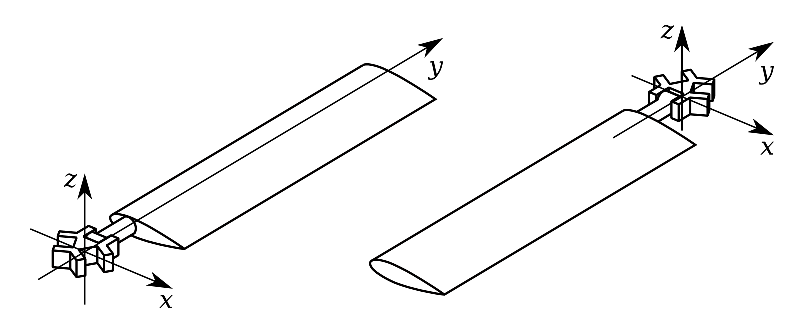
\includegraphics[width=130mm]{eps/coordinate_system_SRAS.eps}
  \caption{Shaft-Rotating Axis System (left CCW, right CW)}
\end{figure}

\begin{figure}
  \centering
  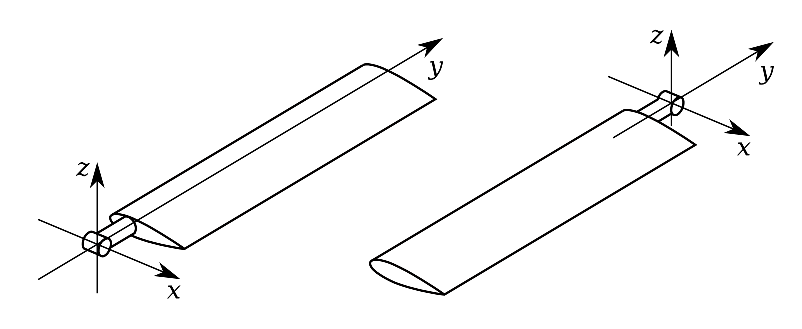
\includegraphics[width=130mm]{eps/coordinate_system_BSAS.eps}
  \caption{Blade-Span Axis System (left CCW, right CW)}
\end{figure}

\begin{equation}
  \boldsymbol T \left( \Psi \right)
  =
  \left[
    \begin{matrix}
      -1 & 0 &  0 \\
       0 & 1 &  0 \\
       0 & 0 & -1 \\
    \end{matrix}
  \right]
  \left[
    \begin{matrix}
       \cos \Psi & \sin \Psi & 0 \\
      -\sin \Psi & \cos \Psi & 0 \\
               0 &         0 & 1 \\
    \end{matrix}
  \right]
  =
  \left[
    \begin{matrix}
      -\cos \Psi & -\sin \Psi &  0 \\
      -\sin \Psi &  \cos \Psi &  0 \\
               0 &          0 & -1 \\
    \end{matrix}
  \right]
\end{equation}
